\documentclass{article}

\usepackage[margin=1in]{geometry}
\usepackage{amsmath}
\usepackage{graphicx}
\usepackage{multicol}
\usepackage{fancyvrb}
\usepackage{bibentry}
\usepackage[shortlabels]{enumitem}
\usepackage{tikz}

\newcommand{\fig}[3]{ 
	\begin{figure}[h]
		\centering
		\caption{#3}
		\includegraphics[width=#2\textwidth]{pics/#1}
		\label{fig:#1}
	\end{figure} 
}

\begin{document}
\title{ESOF 422 - Homework 6}
\author{Nathan Stouffer}

\maketitle
\newpage
\section*{Question 1}
Question 1 refers to the following graph
	\begin{flalign*}
		\indent & N = \{ 1, 2, 3, 4, 5, 6 \} & \\
		& N_0 = \{ 1 \} \\
		& N_f = \{ 6 \} \\
		& E = \{ (1, 2), (2, 3), (2, 6), (3, 4), (3, 5), (4, 5), (5, 2) \} \\
		& def(1) = def(3) = use(3) = use(6) = \{ x \}
	\end{flalign*}
	We also consider the following test paths
	\begin{flalign*}
		\indent & t_1 = [ 1, 2, 6 ] & \\
		& t_2 = [ 1, 2, 3, 4, 5, 2, 3, 5, 2, 6 ] \\
		& t_3 = [ 1, 2, 3, 5, 2, 3, 4, 5, 2, 6 ] \\
		& t_4 = [ 1, 2, 3, 5, 2, 6 ]
	\end{flalign*}
\begin{enumerate}[(a)]
	\item We depict the graph below
	\begin{center}
		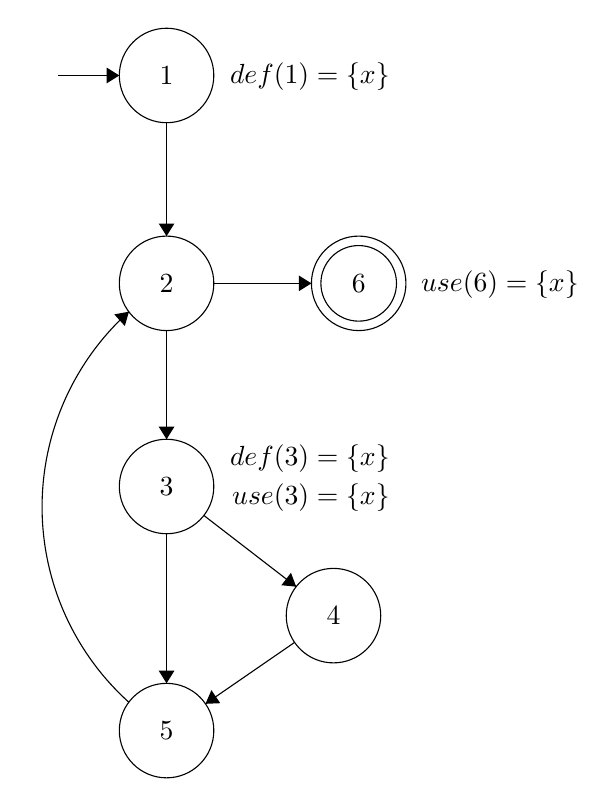
\begin{tikzpicture}[scale=0.2]
		\tikzstyle{every node}+=[inner sep=0pt]
		\draw [black] (36.3,-6.2) circle (3);
		\draw (36.3,-6.2) node {$1$};
		\draw [black] (36.3,-19.4) circle (3);
		\draw (36.3,-19.4) node {$2$};
		\draw [black] (36.3,-32.3) circle (3);
		\draw (36.3,-32.3) node {$3$};
		\draw [black] (46.9,-40.5) circle (3);
		\draw (46.9,-40.5) node {$4$};
		\draw [black] (36.3,-47.8) circle (3);
		\draw (36.3,-47.8) node {$5$};
		\draw [black] (48.5,-19.4) circle (3);
		\draw (48.5,-19.4) node {$6$};
		\draw [black] (48.5,-19.4) circle (2.4);
		\draw [black] (29.4,-6.2) -- (33.3,-6.2);
		\fill [black] (33.3,-6.2) -- (32.5,-5.7) -- (32.5,-6.7);
		\draw [black] (36.3,-9.2) -- (36.3,-16.4);
		\fill [black] (36.3,-16.4) -- (36.8,-15.6) -- (35.8,-15.6);
		\draw [black] (36.3,-22.4) -- (36.3,-29.3);
		\fill [black] (36.3,-29.3) -- (36.8,-28.5) -- (35.8,-28.5);
		\draw [black] (39.3,-19.4) -- (45.5,-19.4);
		\fill [black] (45.5,-19.4) -- (44.7,-18.9) -- (44.7,-19.9);
		\draw [black] (38.67,-34.14) -- (44.53,-38.66);
		\fill [black] (44.53,-38.66) -- (44.2,-37.78) -- (43.59,-38.57);
		\draw [black] (36.3,-35.3) -- (36.3,-44.8);
		\fill [black] (36.3,-44.8) -- (36.8,-44) -- (35.8,-44);
		\draw [black] (44.43,-42.2) -- (38.77,-46.1);
		\fill [black] (38.77,-46.1) -- (39.71,-46.06) -- (39.15,-45.23);
		\draw [black] (33.905,-46) arc (-132.08132:-227.91868:16.707);
		\fill [black] (33.91,-21.2) -- (32.98,-21.37) -- (33.65,-22.11);
		\draw (50.5,-6.25) node [left] {$def(1) = \{ x \}$};
		\draw (50.5,-30.5) node [left] {$def(3) = \{ x \}$};
		\draw (50.5,-33) node [left] {$use(3) = \{ x \}$};
		\draw (62.5,-19.5) node [left] {$use(6) = \{ x \}$};
		\end{tikzpicture}
	\end{center}
	\item We now list all of the du-paths with respect to x as the set 
	$$\{ [1, 2, 3], [1, 2, 6],
		 [3, 5, 2, 3], [3, 5, 2, 6],
		 [3, 4, 5, 2, 3], [3, 4, 5, 2, 6] \}$$
	\item We now must determine which du-paths each test path tours. Note that we consider both direct tours and tours with sidetrips. This is displayed in the following table.
		\begin{center}
			\begin{tabular}{|c||c|c|}
				\hline
				Test paths & du-paths covered directly & du-paths covered with sidetrips \\ [1ex] 
				\hline
				$ t_1 = [ 1, 2, 6 ]$ & $ \{ [1, 2, 6] \} $ & \\
				\hline
				$ t_2 = [ 1, 2, 3, 4, 5, 2, 3, 5, 2, 6 ] $ & % test path
					$ \{ [1, 2, 3], [3, 5, 2, 6], [3, 4, 5, 2, 3] \} $ & % directly toured
					$ \{ [1, 2, 6], [3, 4, 5, 2, 6] \} $ \\ % toured with sidetrips
				\hline
				$ t_3 = [ 1, 2, 3, 5, 2, 3, 4, 5, 2, 6 ] $ & % test path
					$ \{ [1, 2, 3], [3, 5, 2, 3], [3, 4, 5, 2, 6] \} $ & % directly toured
					$ \{ [1, 2, 6], [3, 5, 2, 6] \} $ \\ % toured with sidetrips
				\hline
				$ t_4 = [ 1, 2, 3, 5, 2, 6 ] $ & % test path
					$ \{ [1, 2, 3], [3, 5, 2, 6] \} $ & % toured directly 
					$ \{ [1, 2, 6] \} $ \\ % toured with sidepaths
				\hline
			\end{tabular}
		\end{center}
	\item We now give a minimal test set that satisfies \textit{all defs} coverage with respect to $x$ (using only direct tours). \\\\
		We are able to use the given test paths to create the set that satisfies \textit{all defs} coverage. This set is $ \{ t_4 \} = \{ [1, 2, 3, 5, 2, 6] \} $.
	\item We now give a minimal test set that satisfies \textit{ all uses} coverage with respect to $x$ (using only direct tours). \\\\
		We are able to use the given test paths to create the set that satisfies \textit{all uses} coverage. This set is $ \{ t_4 \} = \{ [1, 2, 3, 5, 2, 6] \} $.
	\item We now give a minimal test set that satisfies \textit{all du-paths} coverage with respect to $x$ (using only direct tours). \\\\
		We are able to use the given test paths to create the set that satisfies \textit{all du-paths} coverage. This set is $ \{ t_1, t_2, t_4 \} = \{ [1, 2, 6], [1, 2, 3, 4, 5, 2, 3, 5, 2, 6], [1, 2, 3, 5, 2, 3, 4, 5, 2, 6] \} $.
\end{enumerate}

\newpage
\section*{Question 2}
List all of the clauses for the predicate below
$$ ( G \lor ((m > a) \lor (s \leq o + n)) \land U ) $$
We define a clause to be a predicate without any logical operators. However, this begs the question: what is a predicate? A predicate is an expression that evaluates to either $true$ or $false$. So, the clauses of the above predicate are $ G$, $(m > a)$, $(s \leq o + n)$, and $U$.
\newpage
\section*{Question 3}
For Question 3, we consider the following predicates.
\begin{enumerate}
	\item $ p_1 = a \land (\lnot b \lor c) $
	\item $ p_2 = (a \land b) \lor (b \land c) \lor (a \land c) $
\end{enumerate}

\subsection*{Predicate 1}
\begin{enumerate}[(a)]
	\item The clauses associated with $p_1 = a \land (\lnot b \lor c) $ are $ \{ a, b, c \}$
	\item We now compute and simplify the conditions under which each clause determines $p_1$. The following is when $a$ determines the predicate:
		\begin{flalign*}
			\indent p_{1a} &= (true \land (\lnot b \lor c)) \oplus ( false \land ( \lnot b \lor c ) )  \\
			&= ( \lnot b \lor c ) \oplus false \\
			&= \lnot b \lor c
		\end{flalign*}
	Now when $b$ determines the predicate:
		\begin{flalign*}
			\indent p_{1b} &= (a \land (\lnot true \lor c)) \oplus ( a \land ( \lnot false \lor c ) ) \\
			&= (a \land (false \lor c)) \oplus ( a \land ( true \lor c ) ) \\
			&= (a \land c ) \oplus ( a \land true ) \\
			&= (a \land c ) \oplus a \\
			&= a \land \lnot c
		\end{flalign*}
	And now when $c$ determines:
		\begin{flalign*}
			\indent p_{1c} &= (a \land (\lnot b \lor true )) \oplus ( a \land ( \lnot b \lor false ) ) \\
			&= ( a \land true ) \oplus ( a \land \lnot b ) \\
			&= a \oplus (a \land \lnot b) \\
			&= a \land b
		\end{flalign*}
	\item We now write the truth table. The first column is an enumeration of input values cases. The next three columns are the values of the input clauses. The fifth column is the value of the predicate. The final three columns denote when the value of $p_*$ (where $*$ is replaced with a clause) determines the value of the predicate. Note that the situations where $p_*$ determine each expression match the results found in part b.
		\begin{center}
			\begin{tabular}{|c|c|c|c||c|c|c|c|} 
				\hline
				& $a$ & $b$ & $c$ & $ a \land ( \lnot b \lor c ) $ & $p_a$ & $p_b$ & $p_c$ \\ [1ex] 
				\hline
				1 & T & T & T & T & $*_{a1}$ &  		& $*_{c1}$  \\
				\hline
				2 & T & T & F & F & 		 & $*_{b1}$ & $*_{c1}$  \\
				\hline
				3 & T & F & T & T & $*_{a2}$ & 			&  			\\
				\hline
				4 & T & F & F & T & $*_{a3}$ & $*_{b1}$ &  			\\
				\hline
				5 & F & T & T & F & $*_{a1}$ & 			&  			\\
				\hline
				6 & F & T & F & F &  		 &  		&  			\\
				\hline
				7 & F & F & T & F & $*_{a2}$ &  		&  			\\
				\hline
				8 & F & F & F & F & $*_{a3}$ &  		&  			\\
				\hline
			\end{tabular}
		\end{center}
	\item We now list all pairs of rows from the above table that satisfy General Active Clause Coverage (GACC) with respect to each clause. \\\\
	For clause $a$, we have
		$$ \{ 1, 3, 4 \} \times \{ 5, 6, 7, 8 \} = \{ (1, 5), (1, 6), (1, 7), (1, 8),
			  (3, 5), (3, 6), (3, 7), (3, 8),
			  (4, 5), (4, 6), (4, 7), (4, 8) \} $$
	For clause $b$, there is the set
		$$ \{ 1 \} \times \{ 7, 8 \} = \{ (1, 7), (1, 8) \} $$
	And for clause $c$, we have
		$$ \{ 1, 3 \} \times \{ 2, 6, 8 \} = \{ (1, 2), (1, 6), (1, 8), (3, 2), (3, 6), (3, 8) \} $$
	\item We now list all pairs of rows from the above table that satisfy Correlated Active Clause Coverage (CACC) with respect to each clause. \\\\
	Beginning with clause $a$, we have the set 
		$$ \{ (1, 5), (1, 6), (1, 7), (1, 8),
			  (3, 5), (3, 6), (3, 7), (3, 8),
			  (4, 5), (4, 6), (4, 7), (4, 8) \} $$
	For clause $b$, there is the set
		$$ \{ (1, 7), (1, 8), (2, 3), (2, 4), 
			  (3, 5), (3, 6), (4, 5), (4, 6) \} $$
	And for clause $c$, we have
		$$ \{ (1, 2), (1, 6), (1, 8), (2, 3),
		 	  (3, 6), (3, 8), (4, 5), (4, 7) \} $$
	\item We now list all pairs of rows from the above table that satisfy Restricted Active Clause Coverage (RACC) with respect to each clause.  The situations that satisfy RACC match with the logical restrictions found in part b. \\\\
	For clause $a$, there is $ \{ (1, 5), (3, 7), (4, 8) \} $. \\
	For clause $b$, there is $ \{ (2, 4) \} $. \\
	For clause $c$, there is $ \{ (1, 2) \} $.
\end{enumerate}
\subsection*{Predicate 2}
\begin{enumerate}[(a)]
	\item The clauses associated with $p_2 = (a \land b) \lor (b \land c) \lor (a \land c) $ are $ \{ a, b, c \}$
	\item We now compute and simplify the conditions under which each clause determines $p_2$. The following is when $a$ determines the predicate:
	\begin{flalign*}
		\indent p_{2a} &= ( true \land b ) \lor ( b \land c ) \lor ( true \lor c ) \oplus ( false \land b ) \lor ( b \land c ) \lor ( false \lor c ) \\
		&= b \lor ( b \land c ) \lor c \oplus false \lor ( b \land c ) \lor false \\
		&= b \lor c \oplus b \land c \\
		&= b \oplus c
	\end{flalign*}
	Now when $b$ determines the predicate:
	\begin{flalign*}
		\indent p_{2b} &= ( a \land true ) \lor ( true \land c ) \lor ( a \lor c ) \oplus ( a \land false ) \lor ( false \land c ) \lor ( a \lor c ) \\
		&= a \lor c \lor ( a \land c ) \oplus false \lor false \lor ( a \land c ) \\
		&= a \lor c \oplus a \land c \\
		&= a \oplus c
	\end{flalign*}
	And now when $c$ determines:
	\begin{flalign*}
		\indent p_{2c} &= ( a \land b ) \lor ( b \land true ) \lor ( a \lor true ) \oplus ( a \land b ) \lor ( b \land false ) \lor ( a \lor false ) \\
		&= ( a \land b ) \lor b \lor a \oplus ( a \land b ) \lor false \lor false \\
		&= a \lor b \oplus a \lor b \\
		&= a \oplus b
	\end{flalign*}
	\item We now write the truth table. The first column is an enumeration of input values cases. The next three columns are the values of the input clauses. The fifth column is the value of the predicate. The final three columns denote when the value of $p_*$ (where $*$ is replaced with a clause) determines the value of the predicate. Note that the situations where $p_*$ determine the expression match with the results found in part b.
		\begin{center}
			\begin{tabular}{|c|c|c|c||c|c|c|c|} 
				\hline
				& $a$ & $b$ & $c$ & $ ( a \land b ) \lor ( b \land c ) \lor ( a \land c ) $ & $p_a$ & $p_b$ & $p_c$ \\ [1ex] 
				\hline
				1 & T & T & T & T & 	     & 			&  		   \\
				\hline
				2 & T & T & F & T & $*_{a1}$ & $*_{b1}$ &  		   \\
				\hline
				3 & T & F & T & T & $*_{a2}$ & 			& $*_{c1}$ \\
				\hline
				4 & T & F & F & F & 	 	 & $*_{b1}$ & $*_{c1}$ \\
				\hline
				5 & F & T & T & T & 		 & $*_{b2}$ & $*_{c2}$ \\
				\hline
				6 & F & T & F & F & $*_{a1}$ &  		& $*_{c2}$ \\
				\hline
				7 & F & F & T & F & $*_{a2}$ & $*_{b2}$ &  		   \\
				\hline
				8 & F & F & F & F & 		 &  		&  		   \\
				\hline
			\end{tabular}
		\end{center}
	\item We now list all pairs of rows from the above table that satisfy General Active Clause Coverage (GACC) with respect to each clause. \\\\
	For clause $a$, we have
		$$ \{ 1, 2, 3 \} \times \{ 4, 6, 8 \} = \{ (1, 4), (1, 6), (1, 8),
												   (2, 4), (2, 6), (2, 8),
												   (3, 4), (3, 6), (3, 8) \} $$
	For clause $b$, there is the set
		$$ \{ 1, 2, 5 \} \times \{ 4, 7, 8 \} = \{ (1, 4), (1, 7), (1, 8),
												   (2, 4), (2, 7), (2, 8),
												   (5, 4), (5, 7), (5, 8) \} $$
	And for clause $c$, we have
		$$ \{ 1, 3, 5 \} \times \{ 4, 6, 8 \} = \{ (1, 4), (1, 6), (1, 8), 
												   (3, 4), (3, 6), (3, 8),
												   (5, 4), (5, 6), (5, 8) \} $$
	\item  We now list all pairs of rows from the above table that satisfy Correlated Active Clause Coverage (CACC) with respect to each clause. \\\\
	Beginning with clause $a$, we have the set 
		$$ \{ (1, 6), (1, 7), (1, 8),
			  (2, 6), (2, 7), (2, 8),
			  (3, 6), (3, 7), (3, 8),
			  (4, 5) \} $$
	For clause $b$, there is the set
		$$ \{ (1, 4), (1, 7), (1, 8),
			  (2, 4), (2, 7), (2, 8),
			  (3, 6),
			  (4, 5),
			  (5, 7), (5, 8) \} $$
	And for clause $c$, we have
		$$ \{ (1, 4), (1, 6), (1, 8),
			  (2, 7),
			  (3, 4), (3, 6), (3, 8),
			  (4, 5),
			  (5, 6), (5, 8) \} $$
	\item We now list all pairs of rows from the above table that satisfy Restricted Active Clause Coverage (RACC) with respect to each clause.  The situations that satisfy RACC match with the logical restrictions found in part b. \\\\
	For clause $a$, there is $ \{ (2, 6), (3, 7) \} $. \\
	For clause $b$, there is $ \{ (2, 4), (5, 7) \} $. \\
	For clause $c$, there is $ \{ (3, 4), (5, 6) \} $.
\end{enumerate}

\end{document}